%%%%%%%%%%%%%%%%%%%%%%%%%%%%%%%%%%%%%%%%%
% University Assignment Title Page 
% LaTeX Template
% Version 1.0 (27/12/12)
%
% This template has been downloaded from:
% http://www.LaTeXTemplates.com
%
% Original author:
% WikiBooks (http://en.wikibooks.org/wiki/LaTeX/Title_Creation)
%
% License:
% CC BY-NC-SA 3.0 (http://creativecommons.org/licenses/by-nc-sa/3.0/)
% 
% Instructions for using this template:
% This title page is capable of being compiled as is. This is not useful for 
% including it in another document. To do this, you have two options: 
%
% 1) Copy/paste everything between \begin{document} and \end{document} 
% starting at \begin{titlepage} and paste this into another LaTeX file where you 
% want your title page.
% OR
% 2) Remove everything outside the \begin{titlepage} and \end{titlepage} and 
% move this file to the same directory as the LaTeX file you wish to add it to. 
% Then add \input{./title_page_1.tex} to your LaTeX file where you want your
% title page.
%
%%%%%%%%%%%%%%%%%%%%%%%%%%%%%%%%%%%%%%%%%
%\title{Title page with logo}
%----------------------------------------------------------------------------------------
%	PACKAGES AND OTHER DOCUMENT CONFIGURATIONS
%----------------------------------------------------------------------------------------

\documentclass[10pt]{article}
\usepackage[english]{babel}
\usepackage[utf8x]{inputenc}
\usepackage{amsmath}
\usepackage{graphicx}
\usepackage[colorinlistoftodos]{todonotes}
\usepackage{subfig}
\usepackage{listings}
\usepackage{color}
\usepackage{geometry}
\usepackage{listings}
\usepackage{enumitem}
\usepackage{ stmaryrd }

\geometry{
	a4paper,
	total={210mm,297mm},
	left=20mm,
	right=20mm,
	top=20mm,
	bottom=20mm,
}
\definecolor{dkgreen}{rgb}{0,0.6,0}
\definecolor{gray}{rgb}{0.5,0.5,0.5}
\definecolor{mauve}{rgb}{0.58,0,0.82}

\begin{document}
	
	\begin{titlepage}
		
		\newcommand{\HRule}{\rule{\linewidth}{0.5mm}} % Defines a new command for the horizontal lines, change thickness here
		
		\center % Center everything on the page
		
		%----------------------------------------------------------------------------------------
		%	HEADING SECTIONS
		%----------------------------------------------------------------------------------------
		
		\textsc{\LARGE Université catholique de Louvain}\\[1cm] % Name of your university/college
		\textsc{\Large Ecole Polytechnique de Louvain}\\[0.5cm] % Major heading such as course name


		
		%----------------------------------------------------------------------------------------
		%	TITLE SECTION
		%----------------------------------------------------------------------------------------
		
		\HRule \\[0.4cm]
		{ \huge \bfseries Projet du cadran}\\[0.4cm] % Title of your document
		\HRule \\[1.5cm]
		
		%----------------------------------------------------------------------------------------
		%	AUTHOR SECTION
		%----------------------------------------------------------------------------------------
		
		\begin{minipage}{0.4\textwidth}
			\begin{flushleft} \large
				\emph{Auteur:}\\
				Marie \textsc{Visschers}\\
				Audrey \textsc{Wenders}\\
				Helena \textsc{Russello}\\
				Wojciech \textsc{Grynczel}\\
			\end{flushleft}
		\end{minipage}
		~
		\begin{minipage}{0.4\textwidth}
			\begin{flushright} \large
				\emph{Matricule:} \\
				\textsc{0880-09-00}\\ % Supervisor's Name
				\textsc{3530-10-00}\\ % Supervisor's Name
				\textsc{5569-14-00}\\ % Supervisor's Name
				\textsc{8803-14-00}\\ % Supervisor's Name												
			\end{flushright}
		\end{minipage}\\[2cm]
		
		% If you don't want a supervisor, uncomment the two lines below and remove the section above
		%\Large \emph{Author:}\\
		%John \textsc{Smith}\\[3cm] % Your name
		
		%----------------------------------------------------------------------------------------
		%	DATE SECTION
		%----------------------------------------------------------------------------------------
		
		{\large \today}\\[2cm] % Date, change the \today to a set date if you want to be precise
		
		%----------------------------------------------------------------------------------------
		%	LOGO SECTION
		%----------------------------------------------------------------------------------------
		

		
\includegraphics[scale=0.10]{logo_UCL_NEW_janv2013.JPG}\\[1cm] % Include a department/university logo - this will require the graphicx package

			
\includegraphics[scale=0.20]{EPL_UCL_Logo.jpg}\\[1cm] % Include a department/university logo - this will require the graphicx package	
		%----------------------------------------------------------------------------------------
		
		\vfill % Fill the rest of the page with whitespace
		
	\end{titlepage}
		
		%----------------------------------------------------------------------------------------
		%	Théorie du problème
		%----------------------------------------------------------------------------------------

\newpage
	\section{Théorie du problème}
	Tout d’abord, commençons par définir ce que l’on entend par cadran dans notre projet : un cadran est un cercle gradué par des nombres entiers. Le cadran se lit en commençant par son sommet et en continuant dans le sens horloger.
	
	Définissons également la notion de rotation : une rotation dans un cadran est un déplacement d’une ou plusieurs unités de tous les éléments de ce cadran, l’ordre de ceux-ci restant inchangé.
	
	Soit $l$ le nombre d’éléments dans le cadran et $k$ égal à $l-1$ (k correspond donc à l’indice du dernier élément du cadran (cfr cadran ci-dessous)).
	
	\begin{figure}[h]
		\centering
		\parbox{5cm}{
			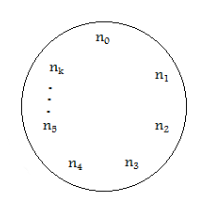
\includegraphics[height=5cm]{1}
			\caption{Le cadran de départ (avant rotation).}
			\label{fig:2figsA}}
		\qquad
		\begin{minipage}{5cm}
			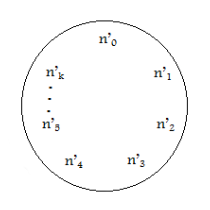
\includegraphics[height=5cm]{2}
			\caption{Le cadran après une rotation de longueur r.}
			\label{fig:2figsB}
		\end{minipage}
	\end{figure}
	
	Après une rotation de longueur r dans un cadran contenant au moins 2 éléments, tous les éléments de celui-ci sont déplacés de r positions vers la droite.
	
	Nous pouvons donc constater que $ \forall l > 1, \forall i \in [0,k]: si\quad i-r \geq 0 \; alors \; n'_i = n_{i-r} \; sinon \; n'_i = n_{l+(i-r)}$
	\\\\
	Exemples:

	\begin{itemize}
		\item Si $ i - r \geq0 $ \\
		Dans cet exemple, $i=$ 4 (c’est $n_4$). Et la rotation $r$ est de 3. Donc pour trouver l’élément $n’_4$ on doit prendre la valeur $n_{i-r}$ c’est-à-dire la valeur $n_1$.
		\begin{figure}[h]
			\centering
			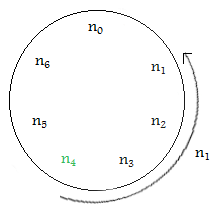
\includegraphics[height=5cm]{3}
			\caption{}
		\end{figure}
		\item Si $ i - r < 0 $ \\
		Dans cet exemple, $i=1$ (c’est $n_1$). Et la rotation $r$ est de 3. Donc pour trouver l’élément $n’_1$, nous remplaçons l’élément $n_1$ par la valeur se trouvant 3 éléments vers la gauche. $n_1 - 3$ nous donne $n_{-2}$ ce qui correspond à la valeur $n_5$ dans le cadran (car $n_5 = n_{l+(i-r)}=n_{7+(-2)}$). $n’_1$ sera donc remplacé par l’élément $n_5$.
		\begin{figure}[h]
			\centering
			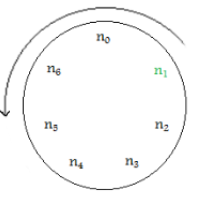
\includegraphics[height=5cm]{4}
			\caption{}
		\end{figure}		
	\end{itemize}
	
	En outre, nous remarquons qu’un cadran vide ou ne contenant qu’un seul élément ne peut pas être soumis à une rotation puisqu’une rotation demande de déplacer plusieurs nombres, or un tableau vide n’en contient pas et un tableau d’un élément n’en contient qu’un.
	
	Nous remarquons également que toute rotation dans un cadran de $n$ éléments dont la longueur $r$ est un multiple de $n$ ne modifiera pas le cadran (cela correspondra à des rotations complètes du cadran). Par exemple, si le cadran contient les nombres 1, 2, 3 et 4 et qu’on effectue une rotation de longueur 4, le cardan finale sera identique au cadran initial. Même chose si on effectue une rotation de 8, 12 ou 28 unités.
	
	$ \forall r, l \in N : si \; l \; mod \; r = 0 \; alors \; \forall i \in [0, k]:n'_i = n_i $ 
	
	De plus, nous pouvons admettre qu’une rotation de longueur r revient à faire une rotation de $r$ modulo $n$. En effet, si $r$ est supérieur ou égal à $n$, les rotations complètes ne sont pas nécessaires (en effet, ci-dessus nous avons constaté que cela ne modifiait pas le cadran), nous pourrons donc nous contenter de faire la rotation $r$ modulo $n$. Et dans le cas où $r$ est inférieur à $n$, nous aurons bien une rotation de $r$ (puisque $\forall r<n: r \; mod \; n = r$).
	
	En nous basant sur les propriétés ci-dessus nous constatons que pour arriver au cadran final, nous effectuons des rotations successives par saut de $r$. Chaque élément est remplacé par l’élément du cadran initial se trouvant $r$ position(s) plus à gauche. Il est donc possible d’arriver au premier élément modifié sans que tous les éléments du cadran aient été déplacés. Typiquement cela arrive lorsque le $pgcd$ de $l$ et de $r$ est inférieur à r.
		\begin{figure}[h]
			\centering
			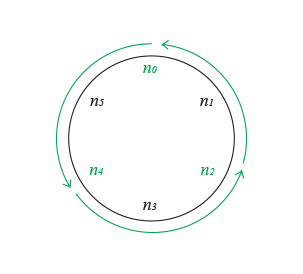
\includegraphics[height=5cm]{5}
			\caption{}
		\end{figure}	

	Pour parvenir à un cadran qui a effectué une rotation de longueur $r$ il faut s’assurer que \underline{tous} les éléments du cadran soient déplacés une seule fois ($O(n)$). De ce fait, lorsque l’on arrive au premier élément placé et que l’on n’a pas déplacé tous les éléments du tableau, on reprend la rotation à partir de l’élément à droite de l’élément courant. Lorsqu’on retournera à ce nouvel élément, si tous les éléments ont été déplacés, le cadran sera bien celui que nous devions obtenir après la rotation, sinon il faudra à nouveau reprendre la rotation à partir de l’élément à droite de l’élément courant et ainsi de suite jusqu’à ce que tous les éléments soient déplacés.
	
	\section{Conventions de représentation (fournies dans le projet)}
	Notre cadran sera représenté par un tableau de nombres entiers Java. Un entier est de type "int" en Java et appartient à [-(2³¹) .. 2³¹ - 1[. Pour construire le tableau à partir du cadran, la convention est de dire que le premier élément du tableau sera l’élément au sommet du cadran. Les éléments suivants sont alors les éléments du cadran dans le sens des aiguilles d’une montre.
	\newpage
	\section{Problème principal}
	Pour ce problème, nous n’avons pas eu besoin de définir des sous-problèmes.
	
	\subsection{Spécifications}
		\begin{description}
			\item[En-tête :] public static void rotate(int[] c, int r)
			\item[Pré :] \begin{description}
							\item $c$ est un tableau d’entiers représentant le cadran à manipuler
							\item $\:$ \&\& $c \neq null $
							\item $\:$ \& $r$ est une entier représentant la rotation réelle à effectuer sur le cadran
							\item  $\:$ \&\& $ r \geq 0 $
						\end{description}
			\item [Post :] le tableau $c$ a été modifié afin de représenter le cadran après rotation de $r$.
			\item [Résultat :] /
		\end{description}

		\begin{description}
			\item[Invariant  :] \begin{description}
				\item $ c \neq null$
				\item $\quad\quad\quad\:\&\&\; r \geq 0$
				\item $\quad\quad\quad\:\&\&\; 0 \leq j \leq c.length $
				\item $\quad\quad\quad\:\&\&\; 0 \leq i \leq nbElemVisite \leq c.length$
				\item $\quad\quad\quad\:\&\&\; -c.length \leq position \leq c.length $ 
			\end{description}
		\end{description}
	\subsection{Construction de l’algorithme}
	
	\begin{lstlisting}
	INIT
	/* INV */
	while(!H)
	ITER
	CLOT
	\end{lstlisting}
	
		\begin{description}
			\item[Variables locales :] int r, i, j, position, tmp, nbElemVisite;
				\item[INIT  :] 
				\begin{description}
					\setlength\itemsep{0.01em}
					\item if c.length = 0
					\item $\quad\quad\quad$ r := 0
					\item $\quad\quad\quad$tmp := 0
					\item $\quad\;$else
					\item $\quad\quad\quad$r := r mod c.length;
					\item $\quad\quad\quad$tmp := c[0];
					\item $\quad\;$i := 0;
					\item $\quad\;$j := i;
					\item $\quad\;$nbElemVisite := 0;
					\item $\quad\;$position := j - r;
				\end{description}		
			\item [H :] $r=0 \;\vee$ nbElemVisite $\geq$ c.length
			\item [ITER  :] 
				\begin{description}
					\setlength\itemsep{0.01em}
					\item if position $<$ 0 
					\item $\quad\quad\quad$ position := position + c.length;
					\item $\quad\;$ if i = position
					\item $\quad\quad\quad$ c[j] := tmp;
					\item $\quad\quad\quad$ i := i + 1;
					\item $\quad\quad\quad$ tmp:= c[i];
					\item $\quad\quad\quad$ j := i;										
					\item $\quad\;$ else
					\item $\quad\quad\quad$ c[j] := c[position];
					\item $\quad\quad\quad$ j := position;
					\item $\quad\;$ nbElemVisite = nbElemVisite + 1;
					\item $\quad\;$ position := j - r;
				\end{description}	
			\item [CLOT :]  /
		\end{description}	
	

	\subsection{Exécutions symboliques}
	
	\subsubsection{\{PRE\} INIT \{INV\}}
	\paragraph{}
	Notons $c_0$ et $r_0$ la valeur des paramètres avant l’exécution de $INIT$.
	
		\setlist[description]{font=\normalfont}
		\begin{description}
			\item[\{$c=c_0, r=r_0$\} tq] \begin{description}
				\item ($c_0$ est un tableau d’entiers représentant le cadran à manipuler
				\item $\quad\quad\quad\quad\quad\quad\:\&\&\; c_0 \neq null$
				\item $\quad\quad\quad\quad\quad\quad\:\&\; r_0$ est une entier représentant la rotation réelle à effectuer sur le cadran
				\item $\quad\quad\quad\quad\quad\quad\:\&\&\; r_0 \geq 0 $)
			\end{description}
		\end{description}
	
	\textbf{if(c.lenght == 0)}
	
	
	\textbf{$\shortdownarrow$ r := 0}
	
		\begin{description}
			\item[\{$c=c_0, r=r_0$\} tq] \begin{description}
				\item ($c_0$ est un tableau d’entiers représentant le cadran à manipuler 
				\item $\quad\quad\quad\quad\quad\quad\:\&\&\; c_0 \neq null$
				\item $\quad\quad\quad\quad\quad\quad\:\&\; r_0$ est une entier représentant la rotation réelle à effectuer sur le cadran
				\item $\quad\quad\quad\quad\quad\quad\:\&\&\; r_0 \geq 0 $
				\item $\quad\quad\quad\quad\quad\quad\:\&\&\; c_o.length = 0)$
			\end{description}
		\end{description}
	
	
	\textbf{$\shortdownarrow$ tmp := 0}
	
	\begin{description}
		\item[\{$c=c_0, r=r_0, tmp=0$\} tq] \begin{description}
			\item ($c_0$ est un tableau d’entiers représentant le cadran à manipuler 
			\item $\quad\quad\quad\quad\quad\quad\:\&\&\; c_0 \neq null$
			\item $\quad\quad\quad\quad\quad\quad\:\&\; r_0$ est une entier représentant la rotation réelle à effectuer sur le cadran
			\item $\quad\quad\quad\quad\quad\quad\:\&\&\; r_0 \geq 0 $
			\item $\quad\quad\quad\quad\quad\quad\:\&\&\; c_o.length = 0)$
		\end{description}
	\end{description}
	
	
	\textbf{$\shortdownarrow$ i := 0}
	
	\begin{description}
		\item[\{$c=c_0, r=r_0, tmp=0, i=0$\} tq] \begin{description}
			\item ($c_0$ est un tableau d’entiers représentant le cadran à manipuler 
			\item $\quad\quad\quad\quad\quad\quad\:\&\&\; c_0 \neq null$
			\item $\quad\quad\quad\quad\quad\quad\:\&\; r_0$ est une entier représentant la rotation réelle à effectuer sur le cadran
			\item $\quad\quad\quad\quad\quad\quad\:\&\&\; r_0 \geq 0 $
			\item $\quad\quad\quad\quad\quad\quad\:\&\&\; c_o.length = 0)$
		\end{description}
	\end{description}	
	
	
	\textbf{$\shortdownarrow$ j := i}
	
	\begin{description}
		\item[\{$c=c_0, r=r_0, tmp=0, i=0, j=0$\} tq] \begin{description}
			\item ($c_0$ est un tableau d’entiers représentant le cadran à manipuler 
			\item $\quad\quad\quad\quad\quad\quad\:\&\&\; c_0 \neq null$
			\item $\quad\quad\quad\quad\quad\quad\:\&\; r_0$ est une entier représentant la rotation réelle à effectuer sur le cadran
			\item $\quad\quad\quad\quad\quad\quad\:\&\&\; r_0 \geq 0 $
			\item $\quad\quad\quad\quad\quad\quad\:\&\&\; c_o.length = 0)$
		\end{description}
	\end{description}	
	

	\textbf{$\shortdownarrow$ nbElemVisite := 0}
	
	\begin{description}
		\item[\{$c=c_0, r=r_0, tmp=0, i=0, j=0, nbElemVisite=0$\} tq] \begin{description}
			\item 
			\item $\quad\quad\quad\quad\quad\quad\:$($c_0$ est un tableau d’entiers représentant le cadran à manipuler 
			\item $\quad\quad\quad\quad\quad\quad\:\&\&\; c_0 \neq null$
			\item $\quad\quad\quad\quad\quad\quad\:\&\; r_0$ est une entier représentant la rotation réelle à effectuer sur le cadran
			\item $\quad\quad\quad\quad\quad\quad\:\&\&\; r_0 \geq 0 $
			\item $\quad\quad\quad\quad\quad\quad\:\&\&\; c_o.length = 0)$
		\end{description}
	\end{description}
	\newpage
	\textbf{$\shortdownarrow$ position := j-r}
	
	\begin{description}
		\item[\{$c=c_0, r=r_0, tmp=0, i=0, j=0, nbElemVisite=0, position=0 $\} tq] \begin{description}
			\item 
			\item $\quad\quad\quad\quad\quad\quad\:$($c_0$ est un tableau d’entiers représentant le cadran à manipuler 
			\item $\quad\quad\quad\quad\quad\quad\:\&\&\; c_0 \neq null$
			\item $\quad\quad\quad\quad\quad\quad\:\&\; r_0$ est une entier représentant la rotation réelle à effectuer sur le cadran
			\item $\quad\quad\quad\quad\quad\quad\:\&\&\; r_0 \geq 0 $
			\item $\quad\quad\quad\quad\quad\quad\:\&\&\; c_o.length = 0)$
		\end{description}
	\end{description}	
	

	\begin{description}
		\item[\underline{Prouver l’invariant} :] \hspace{2pt}
		\begin{itemize}
			\item $ c=c_0$ et $c_0 \neq null → c \neq null $
			\item $ r=0 → r \geq 0 $
			\item $ j=0$ et $c_0.length = 0$ et $c=c_0 → 0 \leq j \leq c.length $
			\item $ i=0$  et $nbElemVisite=0$ et $c_0.length = 0$ et $c=c_0 → 0 \leq i \leq nbElemVisite \leq c.length $
			\item $ position = 0$ et $c_0.length = 0$ et $c=c_0$ et $c_0$ est un tableau ($c.length \geq 0$) \\→  $-c.length \leq position \leq c.length$
		\end{itemize}
		
	\end{description}
	

	\textbf{else // if(c.length != 0)}	
	
		
	\textbf{$\shortdownarrow$ r := r mod c.length}
	
	\begin{description}
		\item[\{$c=c_0, r=r_0$ mod $c_0.length$\} tq] \begin{description}
			\item ($c_0$ est un tableau d’entiers représentant le cadran à manipuler 
			\item $\quad\quad\quad\quad\quad\quad\:\&\&\; c_0 \neq null$
			\item $\quad\quad\quad\quad\quad\quad\:\&\; r_0$ est une entier représentant la rotation réelle à effectuer sur le cadran
			\item $\quad\quad\quad\quad\quad\quad\:\&\&\; r_0 \geq 0 $
			\item $\quad\quad\quad\quad\quad\quad\:\&\&\; c_o.length \neq 0)$
		\end{description}
	\end{description}
	
	\textbf{$\shortdownarrow$ tmp := c[0]}


	\begin{description}
		\item[\{$c=c_0, r=r_0$ mod $c_0.length,  tmp=c_0{[}0{]}$\} tq] 
		\begin{description}
			\item ($c_0$ est un tableau d’entiers représentant le cadran à manipuler 
			\item $\quad\quad\quad\quad\quad\quad\:\&\&\; c_0 \neq null$
			\item $\quad\quad\quad\quad\quad\quad\:\&\; r_0$ est une entier représentant la rotation réelle à effectuer sur le cadran
			\item $\quad\quad\quad\quad\quad\quad\:\&\&\; r_0 \geq 0 $
			\item $\quad\quad\quad\quad\quad\quad\:\&\&\; c_o.length \neq 0)$
		\end{description}
	\end{description}
	
	
	
	\textbf{$\shortdownarrow$ i := 0}
	
	
	\begin{description}
		\item[\{$c=c_0, r=r_0$ mod $c_0.length,  tmp=c_0{[}0{]}, i=0$\} tq] 
		\begin{description}
			\item 
			\item $\quad\quad\quad\quad\quad\quad\:$($c_0$ est un tableau d’entiers représentant le cadran à manipuler 
			\item $\quad\quad\quad\quad\quad\quad\:\&\&\; c_0 \neq null$
			\item $\quad\quad\quad\quad\quad\quad\:\&\; r_0$ est une entier représentant la rotation réelle à effectuer sur le cadran
			\item $\quad\quad\quad\quad\quad\quad\:\&\&\; r_0 \geq 0 $
			\item $\quad\quad\quad\quad\quad\quad\:\&\&\; c_o.length \neq 0)$
		\end{description}
	\end{description}	
	
	
	
	\textbf{$\shortdownarrow$ j := i}
	
	
	\begin{description}
		\item[\{$c=c_0, r=r_0$ mod $c_0.length,  tmp=c_0{[}0{]}, i=0,  j=0$\} tq] 
		\begin{description}
			\item 
			\item $\quad\quad\quad\quad\quad\quad\:$($c_0$ est un tableau d’entiers représentant le cadran à manipuler 
			\item $\quad\quad\quad\quad\quad\quad\:\&\&\; c_0 \neq null$
			\item $\quad\quad\quad\quad\quad\quad\:\&\; r_0$ est une entier représentant la rotation réelle à effectuer sur le cadran
			\item $\quad\quad\quad\quad\quad\quad\:\&\&\; r_0 \geq 0 $
			\item $\quad\quad\quad\quad\quad\quad\:\&\&\; c_o.length \neq 0)$
		\end{description}
	\end{description}		
	
	\newpage
	\textbf{$\shortdownarrow$ nbElemVisite := 0}
	
	
	\begin{description}
		\item[\{$c=c_0, r=r_0$ mod $c_0.length,  tmp=c_0{[}0{]}, i=0,  j=0, nbElemVisite=0$\} tq] 
		\begin{description}
			\item 
			\item $\quad\quad\quad\quad\quad\quad\:$($c_0$ est un tableau d’entiers représentant le cadran à manipuler 
			\item $\quad\quad\quad\quad\quad\quad\:\&\&\; c_0 \neq null$
			\item $\quad\quad\quad\quad\quad\quad\:\&\; r_0$ est une entier représentant la rotation réelle à effectuer sur le cadran
			\item $\quad\quad\quad\quad\quad\quad\:\&\&\; r_0 \geq 0 $
			\item $\quad\quad\quad\quad\quad\quad\:\&\&\; c_o.length \neq 0)$
		\end{description}
	\end{description}		
	
	
	\textbf{$\shortdownarrow$ position := j-r}
	
	
	\begin{description}
		\item[\{$c=c_0, r=r_0$ mod $c_0.length,  tmp=c_0{[}0{]}, i=0,  j=0, nbElemVisite=0, position=0$\} tq] 
		\begin{description}
			\item 
			\item $\quad\quad\quad\quad\quad\quad\:$($c_0$ est un tableau d’entiers représentant le cadran à manipuler 
			\item $\quad\quad\quad\quad\quad\quad\:\&\&\; c_0 \neq null$
			\item $\quad\quad\quad\quad\quad\quad\:\&\; r_0$ est une entier représentant la rotation réelle à effectuer sur le cadran
			\item $\quad\quad\quad\quad\quad\quad\:\&\&\; r_0 \geq 0 $
			\item $\quad\quad\quad\quad\quad\quad\:\&\&\; c_o.length \neq 0)$
		\end{description}
	\end{description}	
	

	
	\begin{description}
		\item[\underline{Prouver l’invariant} :] \hspace{2pt}
		\begin{itemize}
			\item $ c=c_0$ et $c_0 \neq null → c \neq null $
			\item $ r=r_0$ mod $c_0.length$ et $r_0 \geq 0$ et $c_0.length \neq 0$ et $c_0$ est un tableau d’entiers représentant le cadran à manipuler\\
			→ La longeur d’un tableau (ici $c_0$) est forcément $\geq$ à 0. Comme $c_0.length \neq 0$
			, on peut dire que $c_0.length > 0$. Sachant que: $\forall x \geq 0, \forall y > 0: x \mod{y} \geq 0$, sachant que $c_0.lenght > 0$ et $r_0 \geq 0$ nous pouvons dire que $r_0 \mod{c_0.length} \geq 0$ donc $r \geq 0$.
			\item $j=0$ et $c_0.length \neq 0$ et $c=c_0$ et $c_0$ est un tableau d’entiers représentant le cadran à manipuler\\
			→ $0 \leq j \leq c.length$  (car la longueur d’un tableau non vide est forcément supérieure à 0)
			\item $i=0$ et $nbElemVisite=0$ et $c_0.length \neq 0$ et $c=c_0$ et $c_0$ est un tableau d’entiers représentant le cadran à manipuler\\
			→ $0 \leq i \leq nbElemVisite \leq c.length$  (car la longueur d’un tableau non vide est forcément supérieure à $0$)
			\item $position = 0$ et $c_0.length = 0$ et $c=c_0$  et $c_0$ est un tableau ($c.length \geq 0$)\\
			→  $-c.length \leq position \leq c.length$
		\end{itemize}
	\end{description}	
	
	
	L’invariant est vérifié pour les 2 conditions.
	Notons désormais que $0 \leq r \leq c.length$. En effet,$\forall x \geq 0, \forall y > 0 : x \mod{y} \leq y $. Par conséquent,$ r_0 \mod{c_0.length} \leq c_0.length=c.length$ à la fin de l’$INIT$. C’est aussi vrai dans le cas où $r_0=0$ puisque $c_0.length \geq 0$.
	
	
	
	\subsubsection{\{INV \&\& !H\} ITER \{INV\} :}	
	
	$c \neq null\\ 
	\&\&\; r \geq 0\\
	\&\&\; 0 \leq j \leq c.length\\
	\&\&\; 0 \leq i \leq nbElemVisite \leq c.length\\
	\&\&\; -c.length \leq position \leq c.length\\
	\&\&\; (r \neq 0 \;\&\&\; nbElemVisite < c.length)       //!H$
	
	
	
	\begin{description}
		\item Nous commençons par prouver que l’évaluation de la condition d’arrêt ne conduit pas à une erreur si l’invariant est vrai :
		\begin{itemize}
			\item L’invariant impose une condition sur $r$. Cela veut implicitement dire que $r$ est initialisée. Il n’y a donc pas d’erreur lors de l’évaluation de la première partie de la condition d’arrêt.
			\item Supposons que $r=0$, la condition d’arrêt est vraie et la deuxième partie de la condition d’arrêt n’est pas évaluée. L’invariant nous dit que $r \geq 0$, il n’y a donc pas d’erreur d’exécution.
			\item Supposons que $r \neq 0$, alors la condition $r \geq 0$ de l’invariant implique que $r>0$. On évalue alors la deuxième partie de la condition d’arrêt qui vérifie si $nbElemVisite \geq c.length$. Si cette condition est vérifiée, en la combinant avec l’invariant nous obtenons $nbElemVisite = c.length$, ce qui implique qu’il n’y aura pas d’erreur d’exécution.
		\end{itemize}
	\end{description}		
	
	
	Passons maintenant à l’exécution symbolique. Notons $i_1$ la valeur de $i$ avant l’exécution de $ITER$ (idem pour les autres variables). Nous simplifions un peu $\{INV \;\&\&\; !H\}$, et ajoutons la condition trouvée après l’exécution d’$INIT$ ($r_1 \leq c_1.length$ nous pouvons convenir que cela restera vrai si nous prouvons à la fin de l’exécution symbolique que $r=r_1$). Nous obtenons alors les conditions vraies suivantes :	\\	
	
	
	$c_1 \neq null \\
	\&\&\; 0<r_1 \leq c_1.length\quad\quad\quad\quad\quad\quad\quad\quad\quad	      (1)\\
	\&\&\; 0 \leq j_1 \leq c_1.length\\
	\&\&\; 0 \leq i_1 \leq nbElemVisite1 < c_1.length \quad (2)\\
	\&\&\; -c.length \leq position_1 \leq c_1.length$
	

	Notons que $(1)$ et $(2)$ résultent non seulement de l’invariant mais aussi du fait que la condition d’arrêt est fausse.

	
	\begin{description}
		\item \underline{Cas 1} : $position < 0$
			\begin{description}
				\item \{$position=position_1$\}
				\item \quad\quad\quad $\shortdownarrow$$position := position + c.length$
				\item \{$position=position_1+c_1.length$\}
			\end{description}
		\begin{itemize}
			\item $-c.length \leq position \leq c.length$
				\begin{itemize}
					\item[$\circ$] cette condition est vérifiée puisque nous sommes dans le cas où $position_1<0$, nous savons que $c_1.length \geq 0$ (en effet, la longueur d’un tableau ne peut pas être inférieure à $0$) et nous savons que  $-c_1.length \leq position_1 \leq c_1.length$. \\
					Donc $-c.length \leq position = position_1+c_1.length \leq c1.length = c.length$  
					Comme $-c_1.length \leq position_1 \leq c_1.length$ et 
					$position=position_1+c_1.length$ on sait pour la suite que $position \geq 0$.				
				\end{itemize}
		\end{itemize}				
	\end{description}
	
	Pour la suite nous noterons $position_2$ la position après l’execution du cas 1 c’est à dire $position=position_1+c_1.length$. Pour rappel $0 \leq position_2 \leq c_1.length$.
	
	
	\begin{description}
		\item \underline{Cas 2a} : $i = position$		
	\end{description}	
	
	\{$i = i_1, j=j_1,r = r_1, tmp = tmp_1,c{[}j_1{]} = c_1{[}j{]}, nbElemVisite=nbElemVisite_1, position=position_2$\}\\
	\begin{description}
		\item \textbf{$\shortdownarrow \textbf{c{[}j{]} := tmp}$}	
	\end{description}

	
	\{$i = i_1, j=j_1,r = r_1, tmp = tmp_1,c{[}j_1{]} = tmp_1, nbElemVisite=nbElemVisite_1, position=position_2$\}\\	

	\begin{description}
		\item \textbf{$\shortdownarrow \textbf{i := i+1}$}
	\end{description}
		
	\{$i = i_1 + 1, j=j_1,r = r_1, tmp = tmp_1,c{[}j_1{]} = tmp_1, nbElemVisite=nbElemVisite_1, position=position_2$\}\\			
	
	
	\begin{description}
		\item \textbf{$\shortdownarrow \textbf{tmp := c{[}i{]}}$}
	\end{description}	
	
	\mbox{\{$i = i_1 + 1, j=j_1,r = r_1, tmp = c{[}i_1+1{]},c{[}j_1{]} = tmp_1, nbElemVisite=nbElemVisite_1, position=position_2$\}}\\	
	
	
	\begin{description}
		\item \textbf{$\shortdownarrow \textbf{nbElemVisite := nbElemVisite +1}$}
	\end{description}		
	
	\mbox{\{$i = i_1 + 1, j=j_1,r = r_1, tmp = c{[}i_1+1{]},c{[}j_1{]} = tmp_1, nbElemVisite=nbElemVisite + 1, position=position_2$\}}\\	
	
	\begin{description}
		\item \textbf{$\shortdownarrow \textbf{position := j - r}$}
	\end{description}		

	\mbox{\{$i = i_1 + 1, j=j_1,r = r_1, tmp = c{[}i_1+1{]},c{[}j_1{]} = tmp_1, nbElemVisite=nbElemVisite + 1, position=i_1 + 1 -r_1$\}}\\
	\newpage
		\begin{itemize}
			\item $c \neq null$
			\begin{itemize}
				\item[$\circ$] $c_1=c$ et $c_1 \neq null$ donc $c \neq null$
			\end{itemize}
			\item $0<r \leq c.length$ nous n’utilisons pas $r(=r_1)$  donc $\{INV \;\&\&\; !H\}$ est vérifié
			\item $0 \leq j \leq c.length$  
			\begin{itemize}
				\item[$\circ$] $\{INV\; \&\&\; !H\}$ nous dit que $0 \leq i_1 \leq nbElemVisite_1 < c_1.length$ donc $0 \leq i_1 < c_1.length$.\\ Comme $j=i_1+1$ et $c_0=c$, nous avons $0 \leq j \leq c_1.length=c.length$.
			\end{itemize}	
			\item $nbElemVisite_1<c_1.length$ et $nbElemVisite = nbElemVisite_1$ et $c_1= c$ donc \{INV\} est vérifié.   
			\item $0 \leq i \leq c.length$
			\begin{itemize}
				\item[$\circ$] $\{INV\; \&\&\; !H\}$ nous dit que $0 \leq i_1 \leq nbElemVisite_1 < c_1.length$. Donc $0 \leq i_1 < c_1.length$.\\ Comme $i=i_1+1$ et $c_0=c$, nous pouvons en conclure que $0 \leq i \leq c.length$ est bien respecté.
			\end{itemize}
			\item $-c.length \leq position \leq c.length$ 		
			\begin{itemize}
				\item[$\circ$] $position=i_1+1-r_1=i-r_1$ et comme $0<r_1 \leq c.length$ et $0 \leq i \leq c.length$ (prouvé ci-dessus) alors $-c.length \leq position \leq c.length$ est bien respecté.
			\end{itemize}				
		\end{itemize}					
		
	\begin{description}
		\item \underline{Cas 2b} : $i < position$		
	\end{description}	
	
	\{$c{[}j_1{]}=c_1{[}j{]}, r=r_1, position=position_2, j=j_1,i=i_1, nbElemVisite=nbElemVisite_1$\}\\
	
	\begin{description}
		\item \textbf{$\shortdownarrow \textbf{c{[}j{]} := c{[}position{]}}$}	
	\end{description}	
	
	\{$c{[}j_1{]}=c{[}position_2{]}, r=r_1, position=position_2, j=j_1,i=i_1, nbElemVisite=nbElemVisite_1$\}\\	
	
	\begin{description}
		\item \textbf{$\shortdownarrow \textbf{j := position}$}	
	\end{description}		
	
	\{$c{[}j_1{]}=c{[}position_2{]}, r=r_1, position=position_2, j=position_2,i=i_1, nbElemVisite=nbElemVisite_1$\}\\	
	
	\begin{description}
		\item \textbf{$\shortdownarrow \textbf{nbElemVisite := nbElemVisite + 1}$}	
	\end{description}		
	
	\mbox{\{$c{[}j_1{]}=c{[}position_2{]}, r=r_1, position=position_2, j=position_2,i=i_1, nbElemVisite=nbElemVisite_1 + 1$\}}\\	

	\begin{description}
		\item \textbf{$\shortdownarrow \textbf{position := j - r}$}	
	\end{description}		


	\mbox{\{$c{[}j_1{]}=c{[}position_2{]}, r=r_1, position=position_2 - r_1, j=position_2,i=i_1, nbElemVisite=nbElemVisite_1 + 1$\}}\\	

	\begin{itemize}
		\item $c \neq null$ idem que cas 2a	
		\item $0 < r \leq c.length$ idem que cas 2a
		\item $0 \leq j \leq c.length$
		\begin{itemize}
			\item[$\circ$] $j=position_2$ et $0 \leq position_2 \leq c_1.length$ donc $0 \leq j \leq c_1.length=c.length$	
		\end{itemize}	  
		\item $0 \leq i \leq c.length$, nous n’utilisons pas $i (=i_1)$ donc $\{INV\; \&\&\; !H\}$ est vérifié
		\item $-c.length \leq position \leq c.length$
		\begin{itemize}
			\item[$\circ$] $position=position_2-r1$. Comme $0 \leq position_2 \leq c_1.length$ et $0 < r_1 \leq c_1.length$, nous pouvons en déduire que $-c_1.length \leq position < c_1.length$ donc nous avons bien prouver que $-c.length \leq position \leq c.length$.
		\end{itemize}		
	\end{itemize}				

\newpage
	\begin{description}
		\item \underline{Cas 2c} : $i > position$		
	\end{description}	

	\mbox{\{$c{[}j_1{]}=c{[}position_2{]}, r=r_1, position=position_2 - r_1, j=position_2,i=i_1, nbElemVisite=nbElemVisite_1 + 1$\}}\\


	\begin{itemize}
		\item $c \neq null$ idem que cas 2b	
		\item $0 < r \leq c.length$ idem que cas 2b
		\item $0 \leq j \leq c.length$
		\begin{itemize}
			\item[$\circ$] $j=position_2$ et $0 \leq position_2 \leq c_1.length$ donc $0 \leq j \leq c_1.length=c.length$	
		\end{itemize}	
		\item $0 \leq i \leq c.length$ idem que 2b
		\item $-c.length \leq position \leq c.length$ idem que 2b
	\end{itemize}

Nous voyons bien que dans les différents cas $r=r_1$ nous pouvons donc en conclure que la condition $r \leq c.length$ ajoutée dans l’$INIT$ est bien vérifiée.


	\subsubsection{\{INV \&\& H\} CLOT \{POST\} :}	

Les variables $r_2, tmp_2, j_2, i_2, nbElemVisite_2$ et $position_2$ sont les valeurs avant et après $CLOT$ puisque nous sommes dans le cas d’une méthode sans valeur de retour. Il ne se passe rien lors de la clôture.

		\begin{description}
			\item[\{$r=r_2, tmp = tmp_2, j = j_2, i = i_2, nbElemVisite = nbElemVisite_2, position=position_2 $\} tq(] 
			\begin{description}
				\item  
				\item $\quad\quad\quad\quad\quad\quad\: c \neq null$
				\item $\quad\quad\quad\quad\quad\quad\:\&\&\; r \geq 0 $
				\item $\quad\quad\quad\quad\quad\quad\:\&\&\; 0 \leq j \leq c.length$
				\item $\quad\quad\quad\quad\quad\quad\:\&\&\; 0 \leq i \leq nbElemVisite \leq c.length  $
				\item $\quad\quad\quad\quad\quad\quad\:\&\&\; -c.length \leq position \leq c.length$
				\item $\quad\quad\quad\quad\quad\quad\:\&\&\; (r=0 \:||\: nbElemVisite \geq  c.length))$										
			\end{description}
		\end{description}	

	\begin{itemize}
		\item Dans le cas où $r=0$, on sait qu’il n’y a pas de rotation à effectuer (on ne rentre pas dans $ITER$) donc le tableau renvoyé n’a pas été modifié et correspond bien à la clôture: “le tableau $c$ a été modifié afin de représenter le cadran après rotation de $r”$.
		\item Dans le cas où $nbElemVisite = c.length$ (c’est-à-dire $nbElemVisite \geq c.length \;\&\&\; 0 \leq i \leq nbElemVisite \leq c.length$), cela voudra dire que tous les éléments du tableau auront effectué une rotation de $r$. En effet, le nombre d’éléments distincts déplacés ($nbElemVisite$) est égal au nombre d’éléments du tableau ($c.length$). Donc, le tableau renvoyé correspondra également à la clôture.
	\end{itemize}


	\subsubsection{VARIANT}	

	\begin{description}
		\item \underline{Prouver le variant} : ($E$ représente l’environnement)	
		\begin{itemize}	
			\item $INV$ $\implies$ $0 \leq f(E)$\\
			Si l’invariant est vrai, alors $0 \leq nbElemVisite \leq c.length$ 
			donc $0 \leq c.length - nbElemVisite$
			\item $f(E') <f(E)$
		\end{itemize}
	\end{description}	


	\begin{description}
		\item[$E = $\{$r=r_1, tmp=tmp_1,  j=j_1, i=i_1, nbElemVisite=nbElemVisite_1, position=position_1$\} tq(] 
		\begin{description}
			\item  
			\item $\quad\quad\quad\quad\quad\quad\: c \neq null$
			\item $\quad\quad\quad\quad\quad\quad\:\&\&\; r_1 \geq 0 $
			\item $\quad\quad\quad\quad\quad\quad\:\&\&\; 0 \leq j_1 \leq c_1.length$
			\item $\quad\quad\quad\quad\quad\quad\:\&\&\; 0 \leq i_1 \leq nbElemVisite_1 < c_1.length  $
			\item $\quad\quad\quad\quad\quad\quad\:\&\&\; -c_1.length \leq position_1 \leq c_1.length)$									
		\end{description}
	\end{description}	

	\subsubsection{ITER}	

	\begin{description}
		\item[$E' = $\{$..., nbElemVisite=nbElemVisite1+1,...$\} tq(] 
		\begin{description}
			\item  
			\item $\quad\quad\quad\quad\quad\quad\: c \neq null$
			\item $\quad\quad\quad\quad\quad\quad\:\&\&\; r_1 \geq 0 $
			\item $\quad\quad\quad\quad\quad\quad\:\&\&\; 0 \leq j_1 \leq c_1.length$
			\item $\quad\quad\quad\quad\quad\quad\:\&\&\; 0 \leq i_1 \leq nbElemVisite_1 < c_1.length  $
			\item $\quad\quad\quad\quad\quad\quad\:\&\&\; position_1 \leq c_1.length)$									
		\end{description}
	\end{description}	



	($c.length$ n’est pas modifié durant $ITER$)\\
	$Var(E’)=c_1.length-(nbElemVisite_1+1) \leq c_1.length-nbElemVisite_1=Var(E)$.
	C’est vrai puisque $c_1 \neq null$ (donc $c_1.length \geq 0$) 
	et que $0 \leq nbElemVisite_1 < c_1.length$.
	
	Le variant est donc prouvé puisque son résultat est toujours supérieur à $0$ et qu’il décroît à chaque itération.


	\section{Code Java}
	
	\begin{lstlisting}
	public static void rotate(int[] c, int r) {
		// INIT
		int i, j, nbElemVisite, position, tmp;
		if (c.length == 0) {
			r = 0;
			tmp = 0; // valeur sentinelle
		} else {
			r = r % c.length;
			tmp = c[0];
		}
		i = 0; j = i; nbElemVisite = 0; position =  j - r;
		while (r != 0 && nbElemVisite < c.length) { // !H
			// ITER
			if (position < 0) {
				position = position + c.length;
			}
			
			if (i == position) {
				c[j] = tmp;
			
				i++;
				tmp = c[i];
				j = i;
			} else {
				c[j] = c[position];
				j  = position;
			}
			nbElemVisite++;
			position = j - r;
		}
	}
	\end{lstlisting}







				
\end{document}